\begin{center}
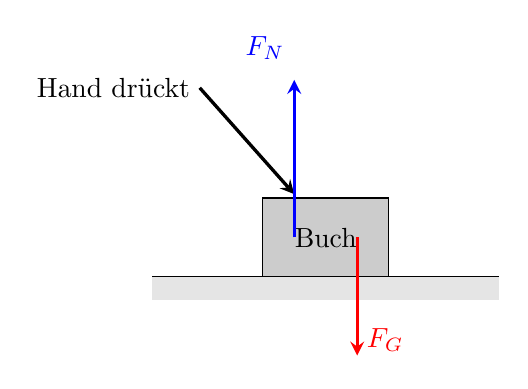
\begin{tikzpicture}[>=stealth]
 \draw (-2.2,0) -- (2.2,0);
 \fill[gray!20] (-2.2,0) rectangle (2.2,-0.3);
 \draw[fill=gray!40] (-0.8,0) rectangle (0.8,1);
 \node at (0,0.5) {Buch};
 \draw[->, very thick] (-1.6,2.4) -- (-0.4,1.05);
 \node[left] at (-1.6,2.4) {Hand drückt};
 \draw[->, very thick, red] (0.4,0.5) -- (0.4,-1.0);
 \node[red, right] at (0.4,-0.8) {$F_\text{G}$};
 \draw[->, very thick, blue] (-0.4,0.5) -- (-0.4,2.5);
 \node[blue, left] at (-0.4,2.9) {$F_\text{N}$};
\end{tikzpicture}
\end{center}

\emph{Beispiel:} Ein Buch liegt auf dem Tisch, und man drückt zusätzlich mit der Hand von oben darauf. Die Gewichtskraft des Buchs bleibt gleich, die Normalkraft des Tisches auf das Buch wird aber grösser, weil sie nun Gewichtskraft und Handkraft zusammen ausgleichen muss: $F_\text{N} > F_\text{G}$. (Ebenso in einem Lift, der nach oben anfährt.)

Nach dem Wechselwirkungsprinzip sind Kraft und Reaktionskraft aber \emph{immer} gleich gross. Normalkraft und Gewichtskraft können also kein Wechselwirkungspaar sein. Ausserdem greifen beide am selben Körper (dem Buch) an, während Kraft und Reaktionskraft immer an zwei verschiedenen Körpern angreifen.

Die Reaktionskraft zur Gewichtskraft (die Erde zieht das Buch an) ist die Kraft, mit der das Buch die Erde anzieht. Die Reaktionskraft zur Normalkraft (der Tisch stösst das Buch nach oben) ist die Kraft, mit der das Buch auf den Tisch drückt.
